% =============================================================================
%  La Cocina de Kojo — Simulación de Eventos Discretos
%  Informe académico
% =============================================================================
\documentclass[12pt,a4paper]{article}

% ── Codificación y lengua ────────────────────────────────────────────────────
\usepackage[utf8]{inputenc}
\usepackage[T1]{fontenc}
\usepackage[spanish]{babel}

% ── Geometría ────────────────────────────────────────────────────────────────
\usepackage[top=2.5cm, bottom=2.5cm, left=3cm, right=2.5cm]{geometry}

% ── Matemáticas ──────────────────────────────────────────────────────────────
\usepackage{amsmath}
\usepackage{amssymb}

% ── Gráficos ─────────────────────────────────────────────────────────────────
\usepackage{graphicx}
\usepackage{float}
\usepackage{subcaption}

% ── Tablas profesionales ──────────────────────────────────────────────────────
\usepackage{booktabs}
\usepackage{siunitx}
\sisetup{
  table-format        = 2.2,
  table-number-alignment = center,
  detect-all
}
\usepackage{array}

% ── Algoritmos y pseudocódigo ─────────────────────────────────────────────────
\usepackage{algorithm}
\usepackage{algpseudocode}
\renewcommand{\algorithmicrequire}{\textbf{Entrada:}}
\renewcommand{\algorithmicensure}{\textbf{Salida:}}
\floatname{algorithm}{Algoritmo}

% ── Código fuente ─────────────────────────────────────────────────────────────
\usepackage{listings}
\usepackage{xcolor}
\definecolor{codebg}{RGB}{248,248,248}
\definecolor{codeframe}{RGB}{200,200,200}
\definecolor{keyword}{RGB}{0,0,180}
\definecolor{string}{RGB}{163,21,21}
\definecolor{comment}{RGB}{0,128,0}

\lstset{
  language        = Python,
  backgroundcolor = \color{codebg},
  frame           = single,
  rulecolor       = \color{codeframe},
  basicstyle      = \ttfamily\small,
  keywordstyle    = \color{keyword}\bfseries,
  stringstyle     = \color{string},
  commentstyle    = \color{comment}\itshape,
  numbers         = left,
  numberstyle     = \tiny\color{gray},
  breaklines      = true,
  showstringspaces= false,
  tabsize         = 4
}

% ── Tipografía ────────────────────────────────────────────────────────────────
\usepackage{setspace}
\onehalfspacing

% ── Cabeceras ─────────────────────────────────────────────────────────────────
\setlength{\headheight}{14pt}
\usepackage{fancyhdr}
\pagestyle{fancy}
\fancyhf{}
\fancyhead[L]{\small La Cocina de Kojo}
\fancyhead[R]{\small Simulación de Eventos Discretos}
\fancyfoot[C]{\thepage}
\renewcommand{\headrulewidth}{0.4pt}

% ── Hipervínculos (siempre al final, antes de cleveref) ───────────────────────
\usepackage[colorlinks=true, linkcolor=blue!60!black,
            citecolor=green!50!black, urlcolor=blue]{hyperref}
\usepackage{cleveref}

% ── Bibliografía ──────────────────────────────────────────────────────────────
\usepackage[numbers,sort&compress]{natbib}

% ── Comandos personalizados ────────────────────────────────────────────────────
\newcommand{\lam}{\lambda}
\newcommand{\murate}{\mu}
\DeclareMathOperator{\EE}{\mathbb{E}}
\DeclareMathOperator{\VV}{\mathbb{V}}

% =============================================================================
\begin{document}
% =============================================================================

% ── Portada ───────────────────────────────────────────────────────────────────
\begin{titlepage}
  \centering
  \vspace*{2cm}
  {\LARGE\bfseries La Cocina de Kojo\par}
  \vspace{0.5cm}
  {\large Simulación de Eventos Discretos\par}
  \vspace{2cm}
  \rule{\linewidth}{0.5pt}\\[0.4cm]
  {\large Informe del Proyecto\par}
  \rule{\linewidth}{0.5pt}\\[1.5cm]
  {\large Asignatura: Simulación\par}
  \vspace{1cm}
  {\normalsize Facultad de Matemática y Computación\\
   Universidad de La Habana\par}
  \vspace{2cm}
  {\normalsize\today\par}
  \vfill
\end{titlepage}

% ── Tabla de contenidos ───────────────────────────────────────────────────────
\tableofcontents
\newpage

% ── Secciones ─────────────────────────────────────────────────────────────────
% =============================================================================
\section{Introducción}
% =============================================================================

\subsection{Descripción del problema}

La Cocina de Kojo es un puesto de comida rápida ubicado en un centro
comercial, con horario de atención de 10:00 am a 9:00 pm (660 minutos).
El local ofrece dos tipos de productos: sándwiches y sushi.
Para los objetivos de este estudio se asume que existen exclusivamente dos
tipos de consumidores: los que consumen únicamente sándwiches y los que
consumen únicamente productos de sushi.

El sistema experimenta dos períodos de hora pico durante la jornada laboral:
el primero entre las 11:30 am y la 1:30 pm, y el segundo entre las 5:00 pm
y las 7:00 pm.
Fuera de estos períodos la demanda es notablemente menor.
El intervalo de tiempo entre la llegada de un consumidor y el siguiente
se modela como un proceso de Poisson homogéneo por tramos (no homogéneo
globalmente), con distribución exponencial de parámetro $\lambda$:
\begin{itemize}
  \item $\lambda_{\text{pico}} = 0{,}30$ clientes/min durante las horas pico,
  \item $\lambda_{\text{fuera}} = 0{,}17$ clientes/min en el resto de la jornada.
\end{itemize}

El tiempo de preparación de cada pedido depende del tipo de producto y sigue
una distribución Uniforme:
\begin{itemize}
  \item Sándwich: $S_{\text{sand}} \sim \mathcal{U}[3{,}\,5]$ minutos,
  \item Sushi:    $S_{\text{sush}} \sim \mathcal{U}[5{,}\,8]$ minutos,
\end{itemize}
con probabilidad $p = 0{,}5$ de que cada cliente solicite sándwich.

Actualmente, dos empleados trabajan toda la jornada preparando pedidos.
La administración ha recibido quejas de clientes por los tiempos de espera y
desea evaluar si incorporar un tercer empleado durante las horas pico reduciría
significativamente el problema.

\subsection{Objetivos}

El objetivo del estudio es comparar mediante simulación dos políticas de
personal:
\begin{description}
  \item[Escenario A (actual):] 2 empleados activos durante toda la jornada.
  \item[Escenario B (alternativa):] 2 empleados base más 1 empleado adicional
    exclusivamente durante las horas pico.
\end{description}

La \textbf{métrica principal de desempeño} es el porcentaje de clientes que
esperan más de 5 minutos para recibir su pedido durante el transcurso de un
día de trabajo.
Métricas secundarias de interés son el tiempo de espera medio, la longitud
media de la cola y la utilización de los empleados.

\subsection{Variables del sistema}

\Cref{tab:variables} resume las variables de entrada y de salida del modelo.

\begin{table}[H]
  \centering
  \caption{Variables del modelo de simulación.}
  \label{tab:variables}
  \begin{tabular}{llll}
    \toprule
    \textbf{Tipo} & \textbf{Variable} & \textbf{Distribución / Valor} & \textbf{Unidad} \\
    \midrule
    Entrada & Tasa de llegadas (pico)     & $\lambda_p = 0{,}30$          & clientes/min \\
    Entrada & Tasa de llegadas (fuera)    & $\lambda_f = 0{,}17$          & clientes/min \\
    Entrada & Servicio sándwich           & $\mathcal{U}[3,5]$            & min \\
    Entrada & Servicio sushi              & $\mathcal{U}[5,8]$            & min \\
    Entrada & Prob.\ cliente sándwich     & $p = 0{,}5$                   & --- \\
    Entrada & Empleados base              & $c = 2$                       & personas \\
    Entrada & Empleados extra (Esc.\ B)   & $e = 1$ en pico               & personas \\
    \midrule
    Salida  & \% clientes $> 5$ min       & estimada por simulación       & \% \\
    Salida  & Tiempo de espera medio      & estimado por simulación       & min \\
    Salida  & Longitud media de la cola   & estimada por simulación       & clientes \\
    Salida  & Utilización de empleados    & estimada por simulación       & --- \\
    \bottomrule
  \end{tabular}
\end{table}

\newpage
% =============================================================================
\section{Detalles de Implementación}
% =============================================================================

La simulación fue implementada íntegramente en Python~3.13, sin el uso de
librerías de simulación externas (p.ej.\ SimPy), con el objetivo de
exhibir explícitamente cada mecanismo del paradigma de eventos discretos.
El código fuente se organiza en seis paquetes independientes:
\texttt{rng} (generación aleatoria), \texttt{engine} (motor DES),
\texttt{model} (dominio del restaurante), \texttt{metrics} (colección
de estadísticos), \texttt{experiments} (ejecución de réplicas) y
\texttt{analysis} (estadística y visualización).

% ---------------------------------------------------------------------------
\subsection{Generador de números aleatorios (LCG)}
% ---------------------------------------------------------------------------

La base del sistema estocástico es un \textbf{Generador Congruencial Lineal}
(LCG), definido por la recurrencia~\citep{knuth1997art}:
\begin{equation}
  X_{n+1} = (A \cdot X_n + C) \bmod M, \qquad U_n = \frac{X_n}{M},
  \label{eq:lcg}
\end{equation}
con los parámetros de Knuth usados también por la biblioteca estándar de C
en Linux (glibc):
\[
  A = 1\,664\,525, \quad C = 1\,013\,904\,223, \quad M = 2^{32}.
\]
Estos parámetros satisfacen los criterios de Hull--Dobell para período
máximo igual a $M = 4\,294\,967\,296$, garantizando que la secuencia no se
repite dentro de ninguna simulación práctica.

% ---------------------------------------------------------------------------
\subsection{Método de la transformada inversa}
% ---------------------------------------------------------------------------

Todas las variables aleatorias se generan mediante el método de la
transformada inversa, cuya validez se sustenta en la siguiente proposición
\citep{curso_conf2,ross2013simulation}.

\begin{quote}
\textbf{Proposición (Transformada Inversa).}
Sea $U \sim \mathcal{U}(0,1)$.
Para cualquier función de distribución acumulada continua $F$, la variable
aleatoria $X = F^{-1}(U)$ tiene distribución $F$.
\end{quote}

\textit{Demostración.}
Sea $F_X(x) = P[X \le x]$.
Entonces:
\[
  F_X(x) = P\!\left[F^{-1}(U) \le x\right]
          = P\!\left[U \le F(x)\right]
          = F(x), \qquad \square
\]
donde la última igualdad es consecuencia de que $U$ es uniforme en $(0,1)$.

\paragraph{Distribución exponencial.}
Para modelar los tiempos entre llegadas se emplea
$X \sim \operatorname{Exp}(\lambda)$, con función de distribución
$F(x) = 1 - e^{-\lambda x}$.
Invirtiendo:
\begin{equation}
  X = -\frac{1}{\lambda}\ln(U).
  \label{eq:exp}
\end{equation}

\paragraph{Distribución uniforme.}
Los tiempos de preparación siguen
$X \sim \mathcal{U}[a,b]$, con $F(x) = (x-a)/(b-a)$.
La inversión da:
\begin{equation}
  X = a + (b - a)\,U.
  \label{eq:unif}
\end{equation}

% ---------------------------------------------------------------------------
\subsection{Streams independientes y Common Random Numbers (CRN)}
% ---------------------------------------------------------------------------

Para garantizar comparaciones estadísticamente válidas entre escenarios se
implementa la técnica de \textbf{números aleatorios comunes}
(CRN)~\citep{law2015simulation}.
Se mantienen tres streams LCG independientes:
\begin{itemize}
  \item \texttt{arrivals}: genera los tiempos entre llegadas sucesivas,
  \item \texttt{type}: determina si cada cliente pide sándwich o sushi,
  \item \texttt{service}: genera la duración de preparación de cada pedido.
\end{itemize}

Cada stream parte de una semilla separada por $10^6$ posiciones:
\[
  \texttt{seed}_{\text{arrivals}} = s, \quad
  \texttt{seed}_{\text{type}}     = s + 10^6, \quad
  \texttt{seed}_{\text{service}}  = s + 2 \times 10^6.
\]
Con ${\sim}200$ clientes por día y 3 streams, el consumo máximo por réplica
es de ${\approx}600$ números, muy inferior al gap de $10^6$.

El invariante clave del CRN es que el tiempo de servicio de cada cliente se
sortea \emph{en el momento de su llegada}, no cuando inicia el servicio.
Así, el cliente $k$ siempre consume el $k$-ésimo número del stream
\texttt{service} independientemente del escenario.
Esto induce correlación positiva $\rho > 0$ entre las réplicas pareadas de
A y B, reduciendo la varianza del estimador de la diferencia:
\[
  \mathbb{V}(\bar{D}) = \mathbb{V}(\bar{A}) + \mathbb{V}(\bar{B}) - 2\,\operatorname{Cov}(A,B).
\]

% ---------------------------------------------------------------------------
\subsection{Tipos de eventos}
% ---------------------------------------------------------------------------

El modelo define cinco tipos de eventos, descritos en \cref{tab:eventos}.

\begin{table}[H]
  \centering
  \caption{Tipos de eventos del modelo DES de La Cocina de Kojo.}
  \label{tab:eventos}
  \begin{tabular}{lp{9cm}}
    \toprule
    \textbf{Tipo} & \textbf{Descripción y acciones principales} \\
    \midrule
    \textsc{llegada}        & Arribo de un nuevo cliente. Se determina su tipo
                              (Bernoulli) y su tiempo de servicio (Uniforme, al llegar).
                              Si hay servidor libre se asigna; si no, el cliente
                              entra a la cola FIFO.
                              Se programa la siguiente llegada. \\
    \addlinespace
    \textsc{partida}        & Fin del servicio de un cliente. El servidor queda
                              libre. Si la cola no está vacía se atiende al
                              siguiente cliente. Si el empleado está marcado
                              para retiro, se elimina. \\
    \addlinespace
    \textsc{inicio\_pico}   & Comienzo de una hora pico. En el Escenario B se
                              añade el empleado extra; si hay cola, comienza a
                              atender de inmediato. \\
    \addlinespace
    \textsc{fin\_pico}      & Fin de una hora pico. En el Escenario B el empleado
                              extra es marcado para retiro si está ocupado, o
                              retirado inmediatamente si está libre. \\
    \addlinespace
    \textsc{fin\_simulacion}& Cierre del día (t = 660 min). Los servicios en curso
                              se completan; los clientes en cola no reciben servicio. \\
    \bottomrule
  \end{tabular}
\end{table}

% ---------------------------------------------------------------------------
\subsection{Algoritmo del bucle DES}
% ---------------------------------------------------------------------------

El \cref{alg:des} muestra el bucle principal de simulación, fiel al
algoritmo de avance de tiempo por próximo evento descrito
en~\citet{banks2010discrete}.

\begin{algorithm}[H]
\caption{Bucle principal de la simulación DES}
\label{alg:des}
\begin{algorithmic}[1]
\Require configuración $\mathtt{cfg}$, streams $\mathtt{rng}$
\Ensure \texttt{ReplicationResult} con métricas del día
\State Crear empleados base; programar primera \textsc{llegada} y eventos de pico
\While{la lista de eventos futuros (FEL) no está vacía}
  \State $e \gets$ extraer evento de mínimo tiempo de la FEL
  \State Avanzar el reloj: $t \gets e.\mathtt{time}$
  \If{$e$ es \textsc{llegada}}
    \State Sortear tipo de cliente y $s \gets$ tiempo de servicio (Transformada Inversa)
    \State Crear cliente con $\mathtt{arrival\_time} = t$, $\mathtt{service\_time} = s$
    \If{existe servidor libre}
      \State Asignar cliente al servidor; programar \textsc{partida} en $t + s$
    \Else
      \State Encolar cliente; registrar cambio de cola
    \EndIf
    \State Programar siguiente \textsc{llegada} en $t + \operatorname{Exp}(\lambda(t))$
  \ElsIf{$e$ es \textsc{partida}}
    \State Liberar servidor; registrar $\mathtt{departure\_time} = t$
    \If{cola no vacía \textbf{y} $t \le T$}
      \State Desencolar siguiente cliente; asignarlo; programar \textsc{partida}
    \EndIf
  \ElsIf{$e$ es \textsc{inicio\_pico} \textbf{y} $\mathtt{extra\_staff} > 0$}
    \State Crear empleado extra; si hay cola, asignarle cliente inmediatamente
  \ElsIf{$e$ es \textsc{fin\_pico} \textbf{y} $\mathtt{extra\_staff} > 0$}
    \State Marcar empleado extra para retiro (o retirar si está libre)
  \EndIf
\EndWhile
\State \Return $\mathtt{MetricsCollector.summarize}()$
\end{algorithmic}
\end{algorithm}

% ---------------------------------------------------------------------------
\subsection{Proceso de Poisson no homogéneo}
% ---------------------------------------------------------------------------

El proceso de llegadas es un proceso de Poisson no homogéneo con función de
intensidad por tramos constantes \citep{curso_conf2}:
\[
  \lambda(t) = \begin{cases}
    0{,}30 & \text{si } t \in [90,210) \cup [420,540), \\
    0{,}17 & \text{en otro caso.}
  \end{cases}
\]
En la implementación, cada evento \textsc{llegada} programa el siguiente
usando $\lambda(t_{\text{actual}})$: en cuanto el reloj supera una frontera
de pico, la siguiente llegada ya utiliza la tasa correcta.

% ---------------------------------------------------------------------------
\subsection{Cálculo de la longitud media de cola}
% ---------------------------------------------------------------------------

La longitud media de cola se estima como el cociente entre el área bajo la
curva $Q(t)$ (número de clientes en cola en el instante $t$) y la duración
del día $T = 660$ min:
\begin{equation}
  \bar{L}_q = \frac{1}{T}\int_0^T Q(t)\,dt
  \approx \frac{1}{T}\sum_k Q(t_k)\,(t_{k+1} - t_k),
  \label{eq:area_cola}
\end{equation}
donde la suma es una integral de Riemann por rectángulos actualizada en cada
evento de cambio de cola.
Este estimador es equivalente al que se obtiene aplicando la Ley de
Little~\citep{little1961proof}: $L_q = \lambda\,W_q$.

% ---------------------------------------------------------------------------
\subsection{Protocolo de réplicas y parada}
% ---------------------------------------------------------------------------

Se ejecutan $n = 30$ réplicas independientes para cada escenario.
La semilla de la réplica $i$ es $s_i = 42 + i \times 10^5$, garantizando
una separación mayor que el consumo por réplica (${\approx}600$ números).
El criterio de parada formal propuesto en~\citet{curso_temas} (cap.~4) es:
\begin{equation}
  \frac{S}{\sqrt{n}} < d,
  \label{eq:parada_temas}
\end{equation}
donde $d$ es la desviación estándar máxima admisible para el estimador.
Este criterio se analiza en detalle en la \cref{sec:parada}.

\newpage
% =============================================================================
\section{Resultados y Experimentos}
% =============================================================================

% ---------------------------------------------------------------------------
\subsection{Configuración experimental}
% ---------------------------------------------------------------------------

Se ejecutaron 30 réplicas de cada escenario usando números aleatorios comunes
(CRN) con semilla base $s_0 = 42$.
Cada réplica modela un día completo de operación (660 minutos).
La correlación observada entre las réplicas pareadas fue $\hat{\rho} = 0{,}552$,
confirmando la eficacia del CRN.

% ---------------------------------------------------------------------------
\subsection{Tabla de resultados}
% ---------------------------------------------------------------------------

La \cref{tab:resultados} presenta la media y el intervalo de confianza al
95\,\% (distribución $t$ de Student con $n-1 = 29$ grados de libertad) para
cada métrica de salida.

\begin{table}[H]
  \centering
  \caption{Resultados de la simulación --- media e IC~95\,\% (30 réplicas, CRN).}
  \label{tab:resultados}
  \setlength{\tabcolsep}{6pt}
  \begin{tabular}{l
                  S[table-format=2.3]
                  @{\;}
                  l
                  S[table-format=2.3]
                  @{\;}
                  l}
    \toprule
    \textbf{Métrica}
      & \multicolumn{2}{c}{\textbf{Escenario A}}
      & \multicolumn{2}{c}{\textbf{Escenario B}} \\
    \cmidrule(lr){2-3}\cmidrule(lr){4-5}
      & {Media} & {IC 95\,\%}
      & {Media} & {IC 95\,\%} \\
    \midrule
    \% clientes $>$ 5 min      & 16.70 & {[13.69,\;19.72]} & 3.10  & {[2.01,\;4.19]}   \\
    Espera media (min)          & 2.185 & {[1.880,\;2.491]} & 0.658 & {[0.566,\;0.750]} \\
    Espera máxima (min)         & 13.46 & {[12.00,\;14.93]} & 7.37  & {[6.51,\;8.22]}   \\
    Longitud media de cola (clientes) & 0.482 & {[0.408,\;0.556]} & 0.146 & {[0.123,\;0.169]} \\
    Utilización media (\%)      & 57.16 & {[55.67,\;58.66]} & 50.16 & {[48.82,\;51.50]} \\
    \bottomrule
  \end{tabular}
\end{table}

Los intervalos de confianza de ambos escenarios no se solapan en ninguna
métrica, lo cual sugiere diferencias sustanciales; la significancia se
verifica formalmente con el test pareado que se reporta a continuación.

La \cref{fig:dashboard} presenta una visión integrada de los cuatro
indicadores principales.

\begin{figure}[H]
  \centering
  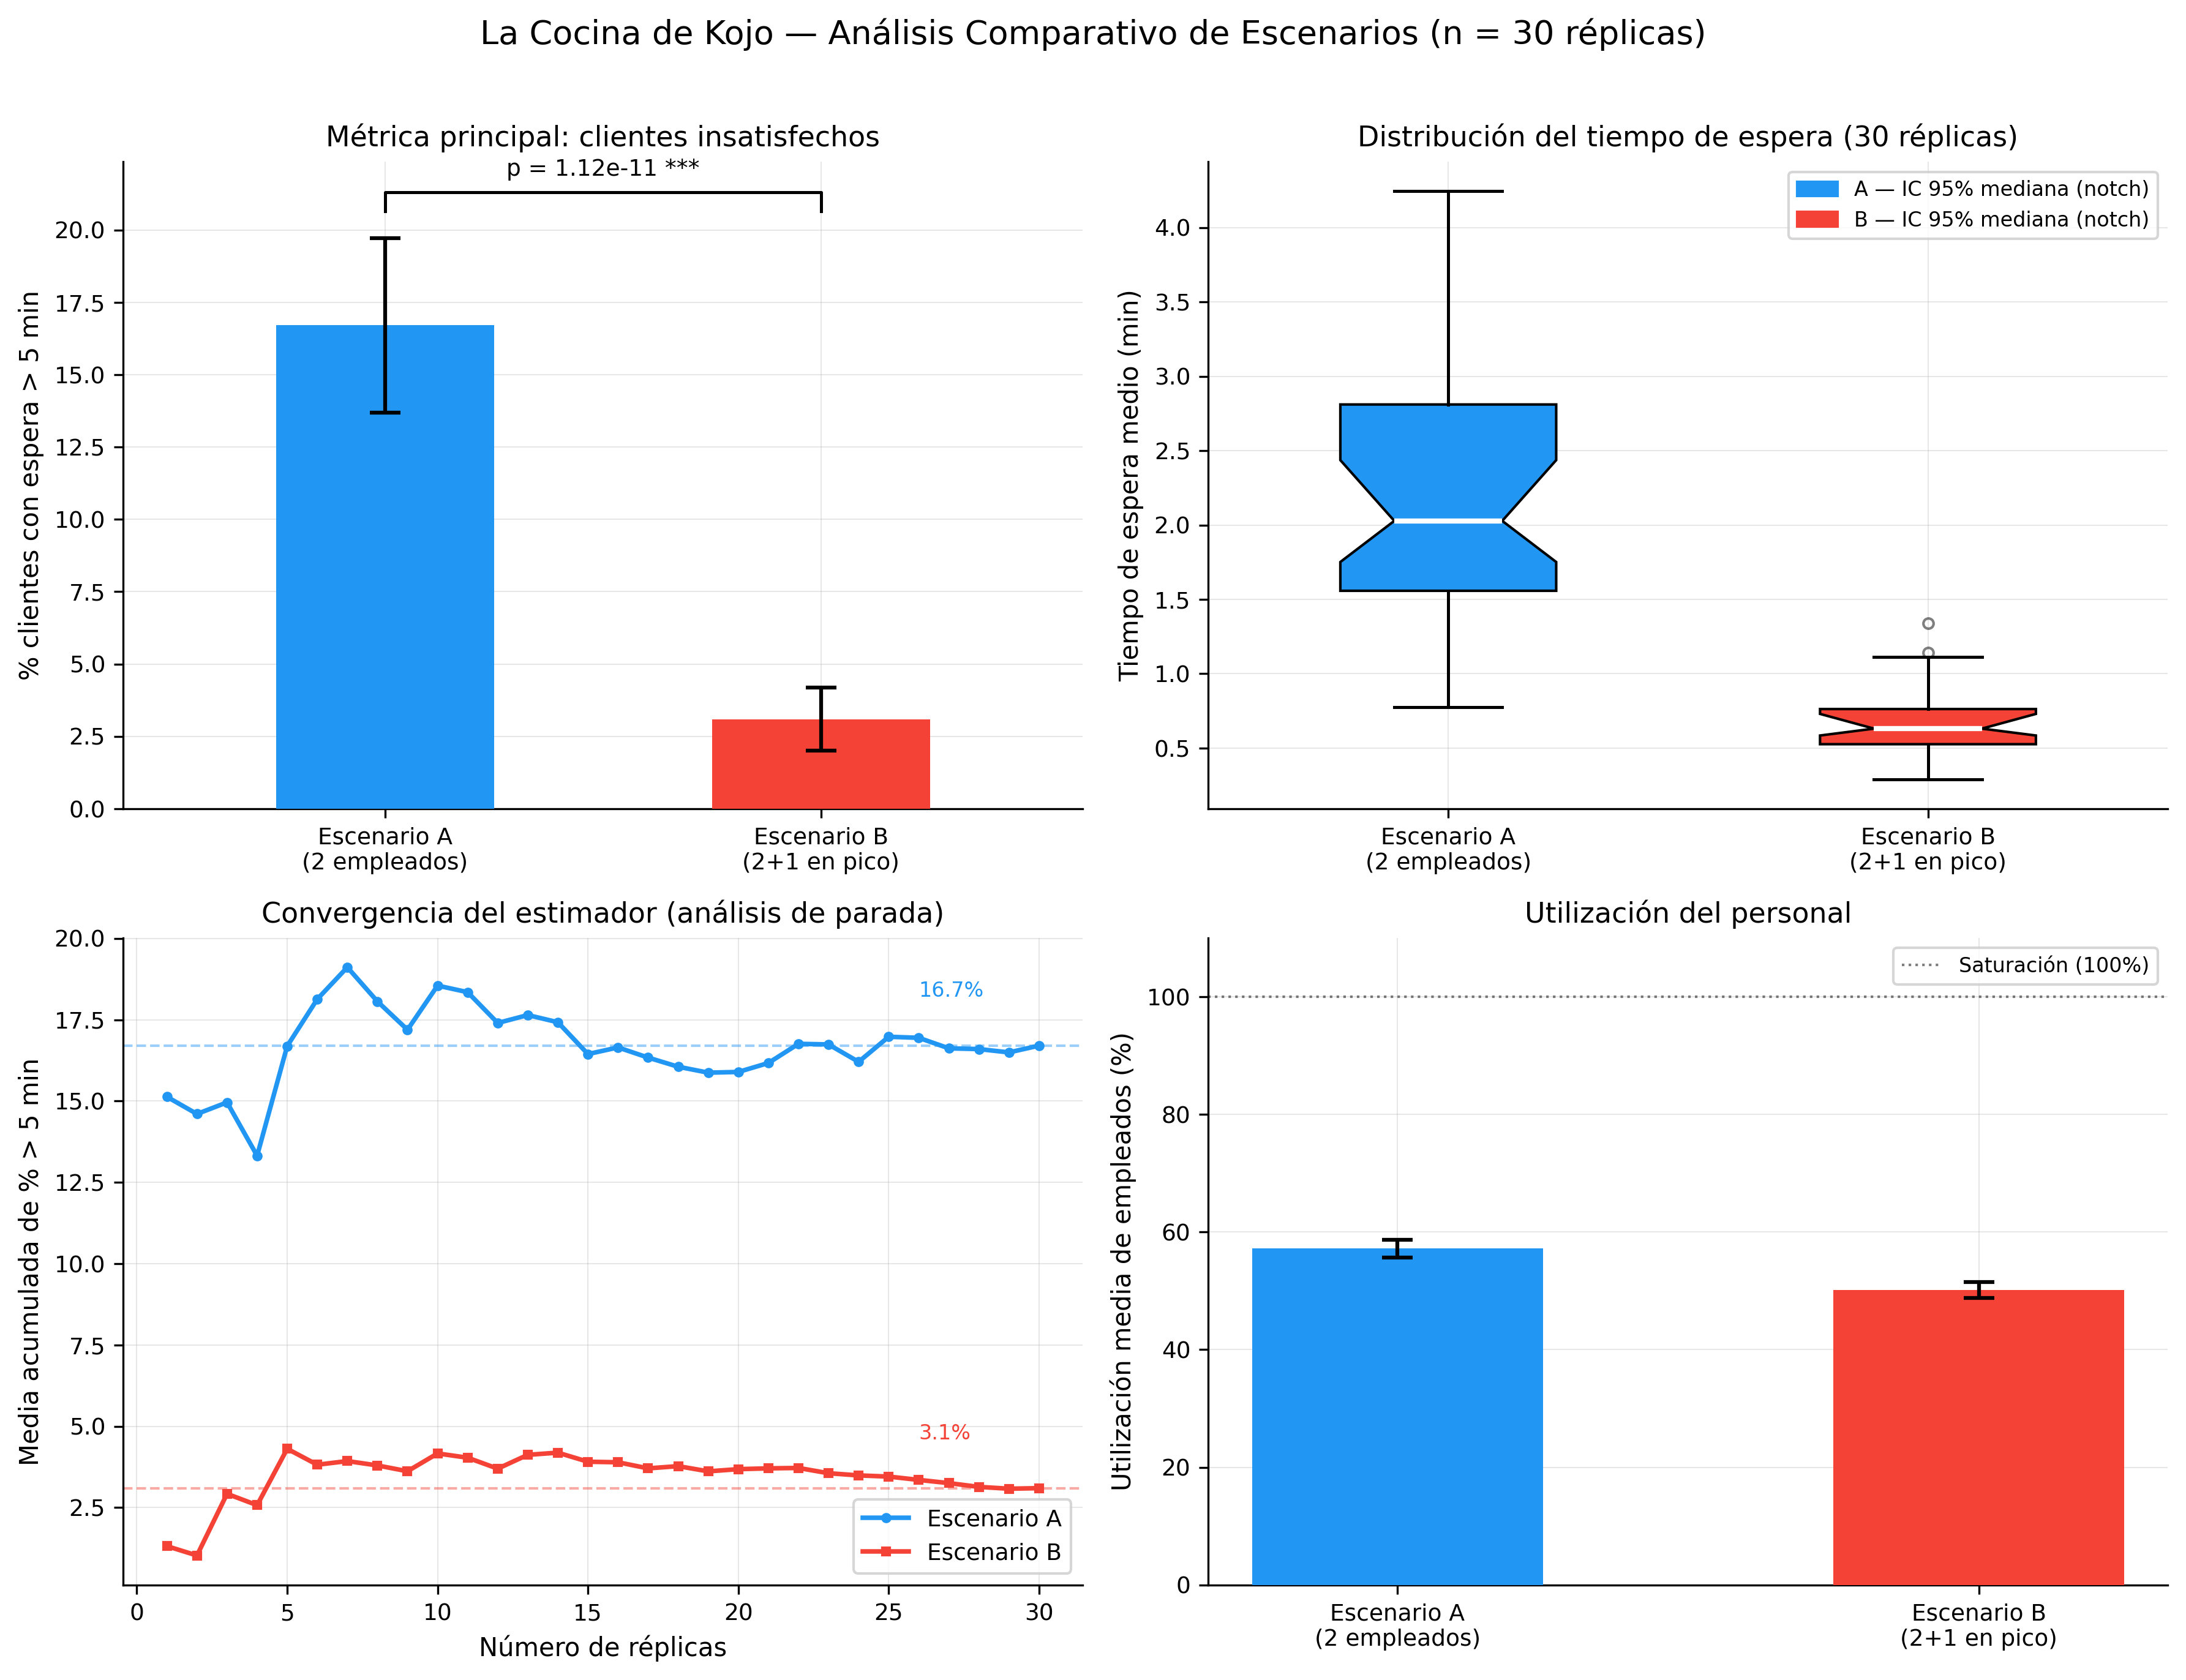
\includegraphics[width=\linewidth]{figures/dashboard.png}
  \caption{Panel comparativo con las cuatro métricas principales.
           Barras de error = IC 95\,\%; notches en box plots = IC 95\,\%
           de la mediana (bootstrap, $B = 5\,000$).}
  \label{fig:dashboard}
\end{figure}

% ---------------------------------------------------------------------------
\subsection{Comparación estadística entre escenarios}
% ---------------------------------------------------------------------------

Se emplea un \textbf{$t$-test pareado} (también llamado test de muestras
relacionadas), ya que las réplicas de A y B están emparejadas por CRN.
El test trabaja sobre las diferencias $D_i = A_i - B_i$:

\[
  H_0: \mu_D = 0
  \qquad \text{vs.} \qquad
  H_1: \mu_D \neq 0,
\]

con estadístico $t = \bar{D} / (S_D / \sqrt{n})$.
Los resultados son:

\begin{center}
\begin{tabular}{ll}
  \toprule
  Diferencia media $\bar{D}$ & $13{,}61$\,\% \\
  IC 95\,\% de $\bar{D}$     & $[11{,}03,\;16{,}18]$\,\% \\
  Estadístico $t$             & $10{,}799$ \\
  $p$-value                   & $1{,}12 \times 10^{-11}$ \\
  Significativo ($\alpha=0{,}05$) & Sí \\
  \bottomrule
\end{tabular}
\end{center}

El intervalo de confianza de la diferencia no contiene el cero.
Se rechaza $H_0$ con un nivel de confianza superior al 99{,}99\,\%:
el tercer empleado reduce significativamente el porcentaje de clientes
insatisfechos.

La \cref{fig:boxplots} muestra la distribución de los tiempos de espera
a través de las 30 réplicas.
Los notches (IC 95\,\% de la mediana) de ambos escenarios no se solapan,
corroborando el test paramétrico con una técnica no paramétrica.

\begin{figure}[H]
  \centering
  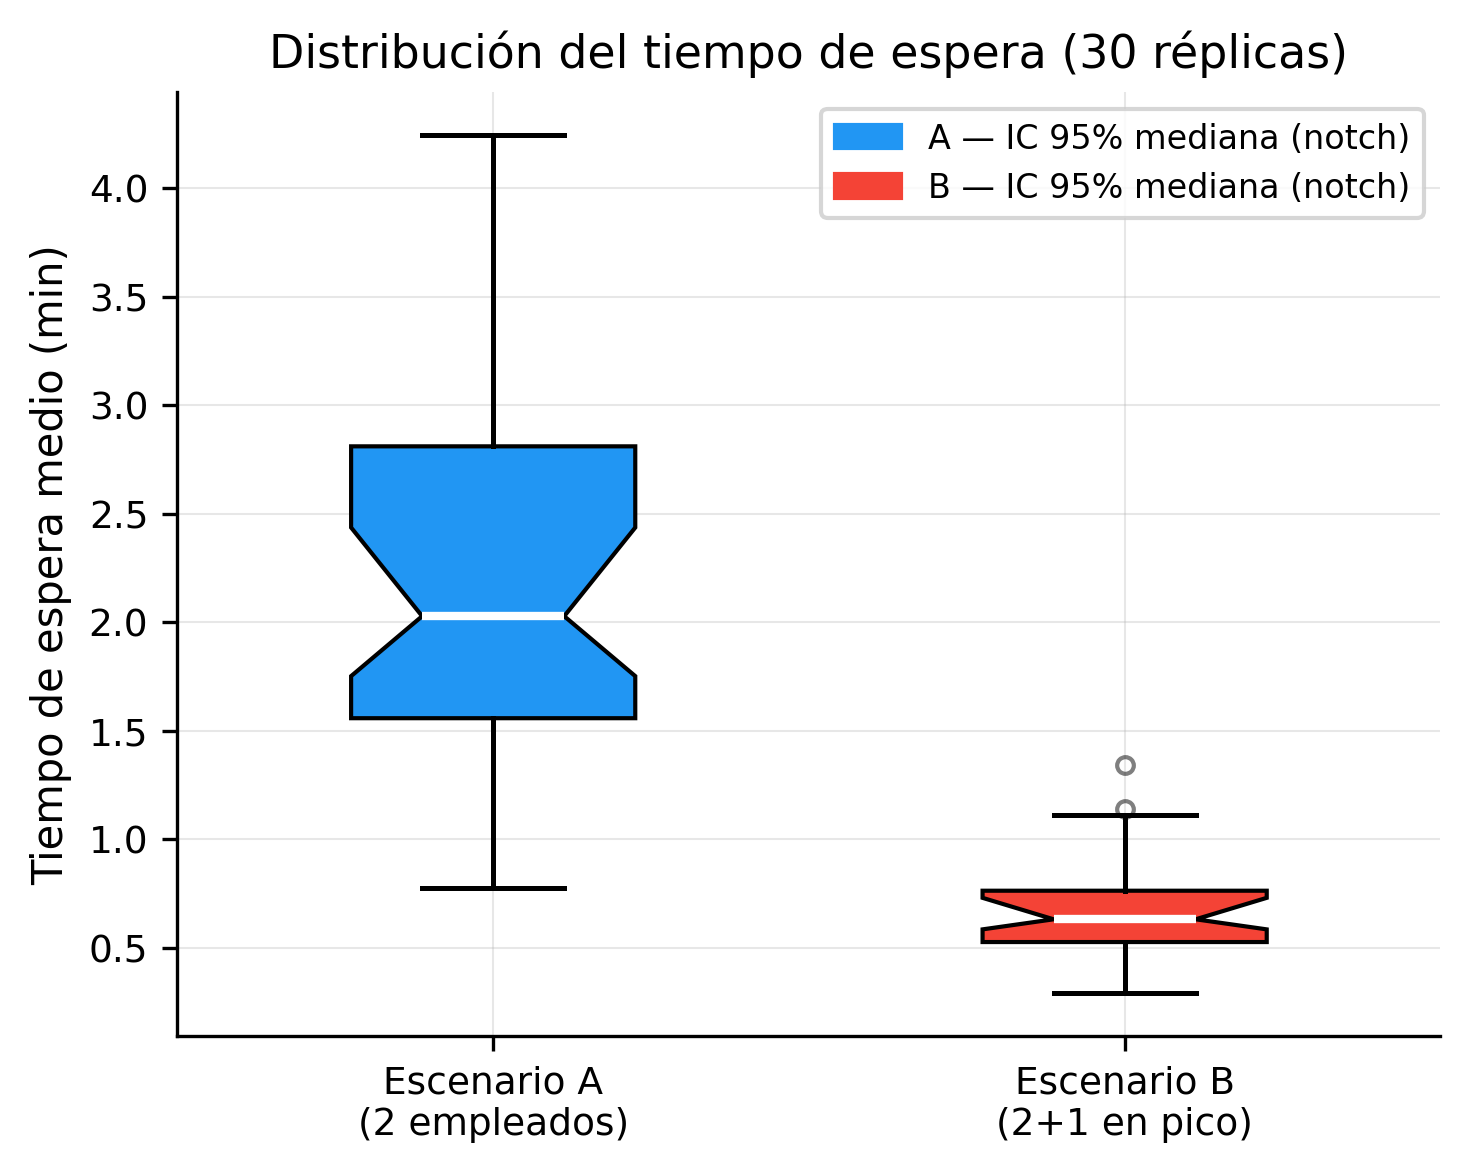
\includegraphics[width=0.7\linewidth]{figures/wait_boxplots.png}
  \caption{Box plots del tiempo de espera medio por réplica.
           Los notches representan el IC 95\,\% de la mediana
           (bootstrap, $B = 5\,000$).}
  \label{fig:boxplots}
\end{figure}

% ---------------------------------------------------------------------------
\subsection{Análisis de parada de la simulación}
\label{sec:parada}
% ---------------------------------------------------------------------------

El criterio de parada de~\citet{curso_temas} establece continuar hasta que
$S/\sqrt{n} < d$.
Equivalentemente, el número mínimo de réplicas para una
precisión relativa $r$ es~\citep{law2015simulation}:
\begin{equation}
  n^* = \left\lceil \left(
    \frac{t_{\alpha/2,\,n-1}\;\hat{S}}{r\;\bar{x}}
  \right)^2 \right\rceil,
  \label{eq:n_star}
\end{equation}
con $r = 0{,}05$ (5\,\% de precisión relativa).

Los resultados de aplicar la~\cref{eq:n_star} son:

\begin{center}
\begin{tabular}{lcccc}
  \toprule
  Escenario & $\bar{x}$ (\%) & $\hat{S}$ (\%) & $n^*$ (5\,\% relativo) & Semi-anchura (\%) \\
  \midrule
  A & 16{,}70 & 8{,}07 & 391  & $3{,}01$ \\
  B &  3{,}10 & 2{,}93 & 1493 & $1{,}09$ \\
  \bottomrule
\end{tabular}
\end{center}

\paragraph{Interpretación.}
El criterio de precisión relativa del 5\,\% no se satisface con 30 réplicas.
Esto se debe a la alta variabilidad intrínseca del indicador: el coeficiente
de variación es $CV_A = 8{,}07 / 16{,}70 \approx 48$\,\% para el Escenario A
y $CV_B = 2{,}93 / 3{,}10 \approx 94$\,\% para el Escenario B.
Un $CV$ tan elevado en el Escenario B es consecuencia de que el porcentaje de
clientes insatisfechos es pequeño (media del 3{,}1\,\%) pero con alta dispersión
entre réplicas: algunos días no se produce ninguna espera larga, mientras que
otros sí.
En estas condiciones, alcanzar una precisión relativa del 5\,\% requeriría del
orden de 400--1500 réplicas.

\paragraph{Precisión absoluta.}
Una forma alternativa de evaluar la suficiencia de las réplicas es mediante la
semi-anchura del IC en términos absolutos.
Con 30 réplicas se obtiene:
\begin{itemize}
  \item Escenario A: IC 95\,\% $= [13{,}69;\;19{,}72]$\,\%, semi-anchura $= 3{,}01$\,\%.
  \item Escenario B: IC 95\,\% $= [2{,}01;\;4{,}19]$\,\%, semi-anchura $= 1{,}09$\,\%.
\end{itemize}
Para la decisión de política de personal, conocer que el Escenario A produce
entre el 13{,}7\,\% y el 19{,}7\,\% de clientes insatisfechos, frente al
2{,}0\,\%--4{,}2\,\% del Escenario B, es más que suficiente.
La diferencia entre ambos intervalos es de varios órdenes de magnitud y no
depende de la estimación puntual exacta.

\paragraph{Suficiencia para la hipótesis principal.}
Aunque la precisión relativa del 5\,\% no se alcanza, el $p$-value de
$1{,}12 \times 10^{-11}$ demuestra que la diferencia entre escenarios es
estadísticamente detectable con garantía absoluta usando 30 réplicas.
El criterio de~\citet{curso_temas} controla la precisión de la \emph{estimación
puntual}; la \emph{detección de diferencias} (objetivo principal del estudio)
requiere potencia estadística, no precisión de estimación, y esa potencia queda
demostrada.
Por tanto, 30 réplicas son suficientes para responder la pregunta de negocio,
aunque se recomendaría aumentarlas si el objetivo fuera reportar el porcentaje
exacto del Escenario B con mayor certeza.

La \cref{fig:convergencia} muestra cómo la media acumulada de cada escenario
se estabiliza alrededor de las réplicas 15--20, confirmando que el estimador
converge dentro del experimento de 30 réplicas.

\begin{figure}[H]
  \centering
  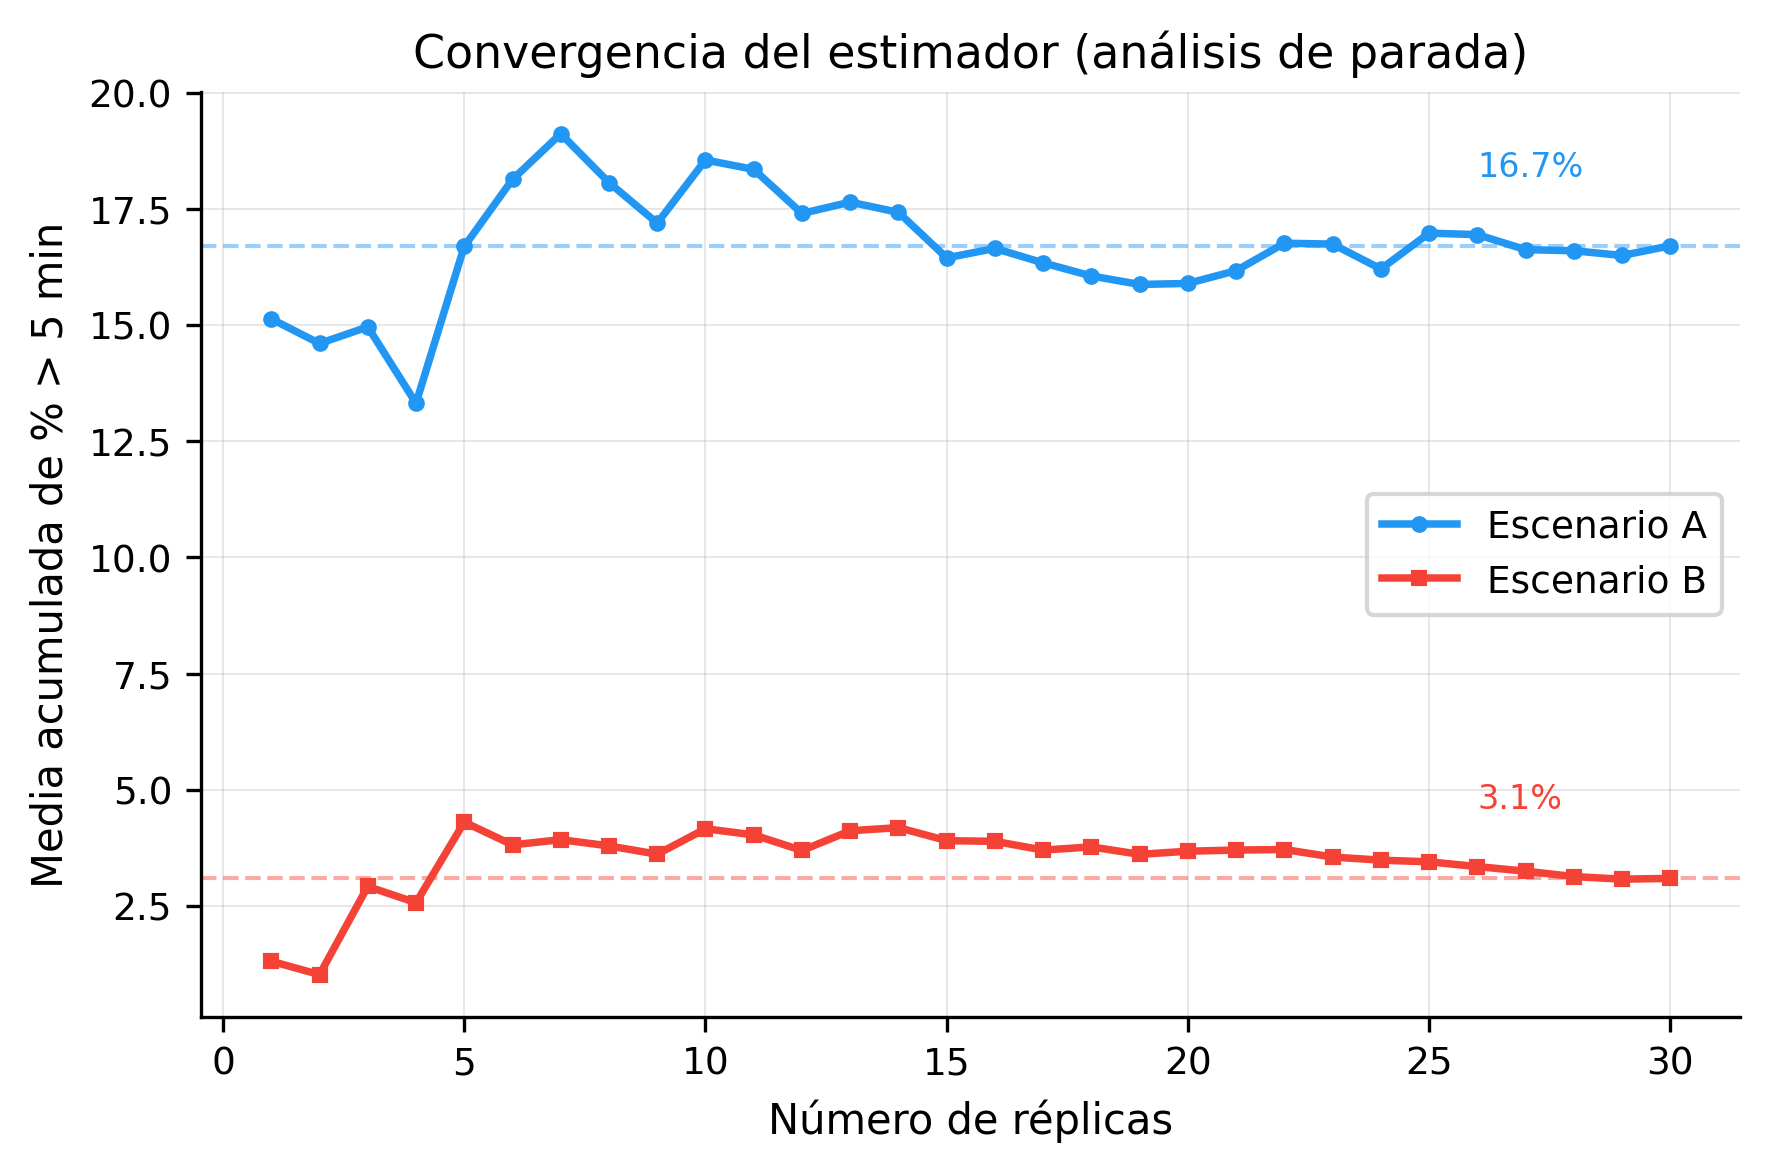
\includegraphics[width=0.85\linewidth]{figures/convergence.png}
  \caption{Convergencia del estimador $\bar{x}_k$ (media acumulada tras $k$
           réplicas). La línea discontinua indica la estimación final.}
  \label{fig:convergencia}
\end{figure}

\begin{figure}[H]
  \centering
  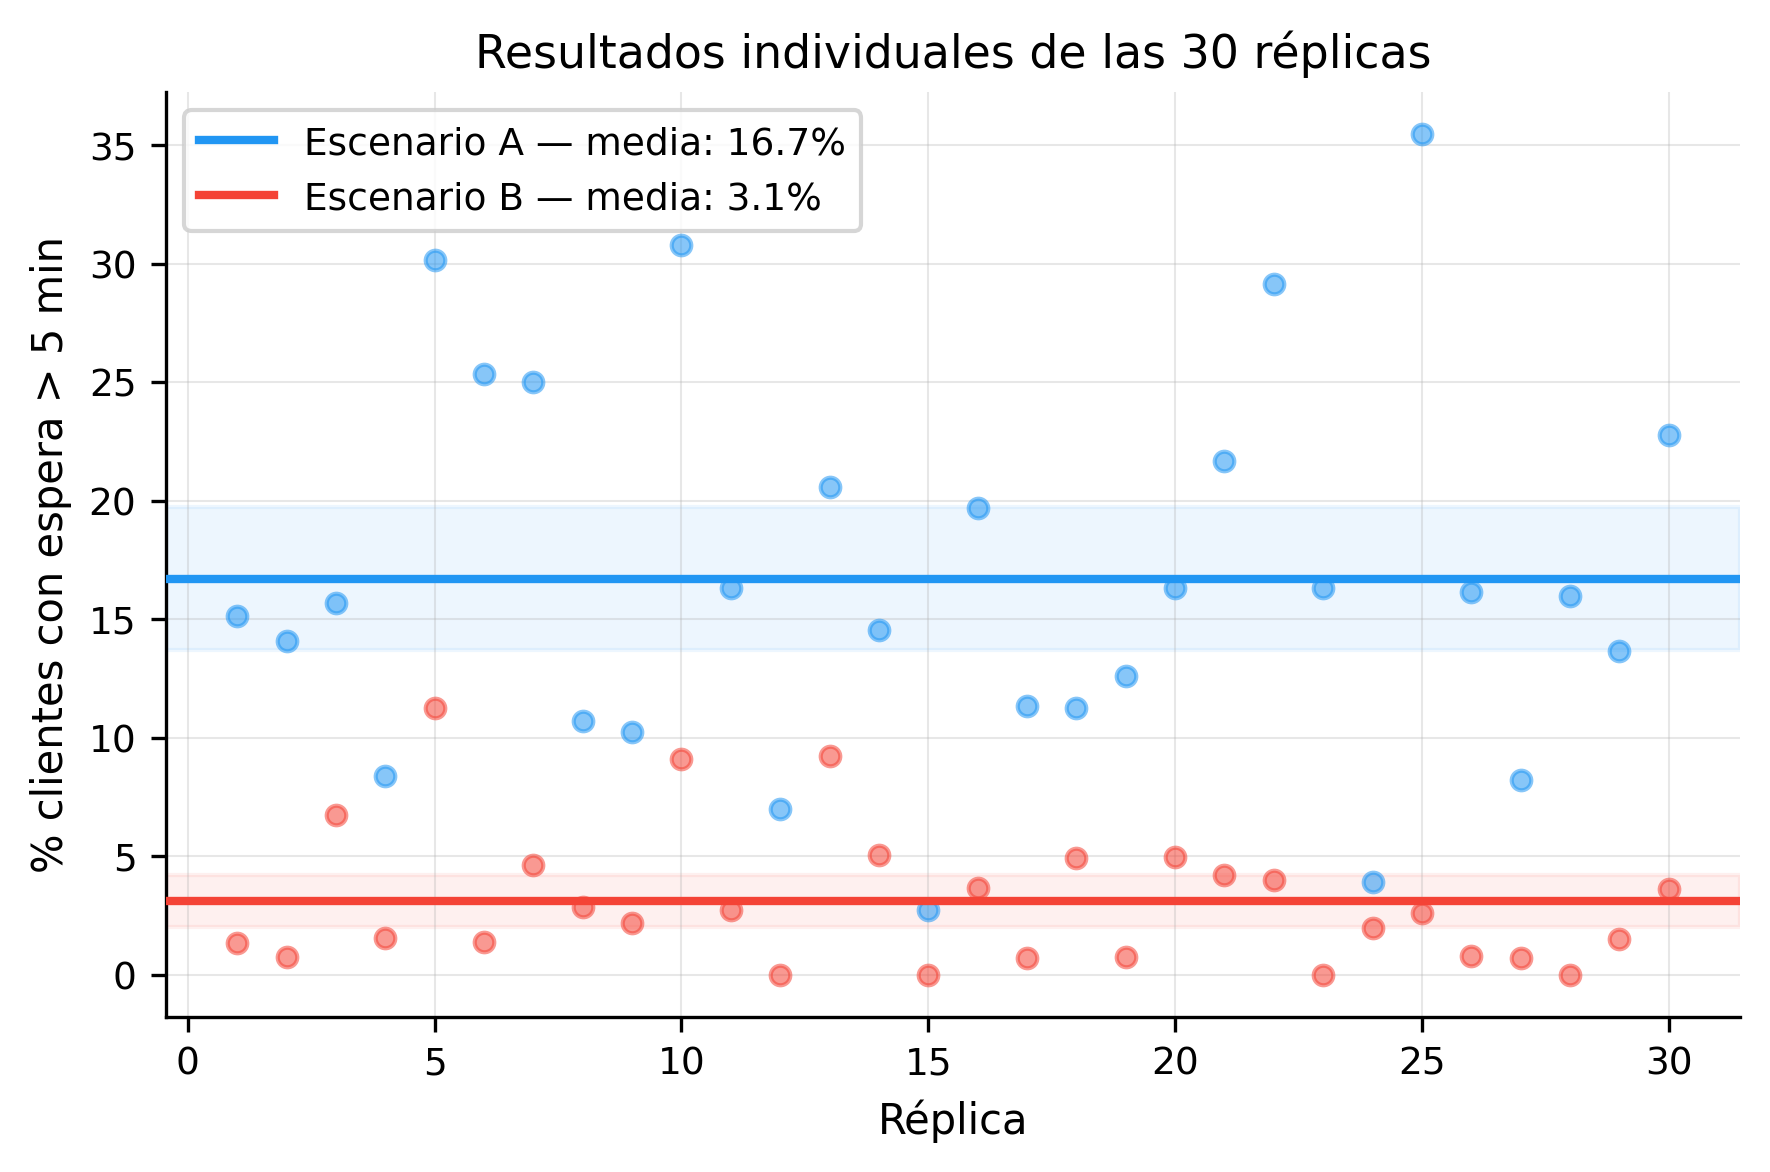
\includegraphics[width=0.85\linewidth]{figures/replication_traces.png}
  \caption{Resultados individuales de las 30 réplicas para cada escenario.
           La línea gruesa es la media; la banda sombreada es el IC~95\,\%.}
  \label{fig:replicas}
\end{figure}

% ---------------------------------------------------------------------------
\subsection{Análisis de sensibilidad}
\label{sec:sensibilidad}
% ---------------------------------------------------------------------------

El enunciado requiere analizar el impacto de la variación de los parámetros
del problema.
Se estudia la sensibilidad de la métrica principal al parámetro más influyente:
la \textbf{tasa de llegadas en hora pico} $\lambda_{\text{peak}}$.

Se ejecutan 10 réplicas por punto para valores
$\lambda_{\text{peak}} \in \{0{,}10,\,0{,}15,\,\ldots,\,0{,}50\}$,
manteniendo constantes el resto de parámetros.

\begin{figure}[H]
  \centering
  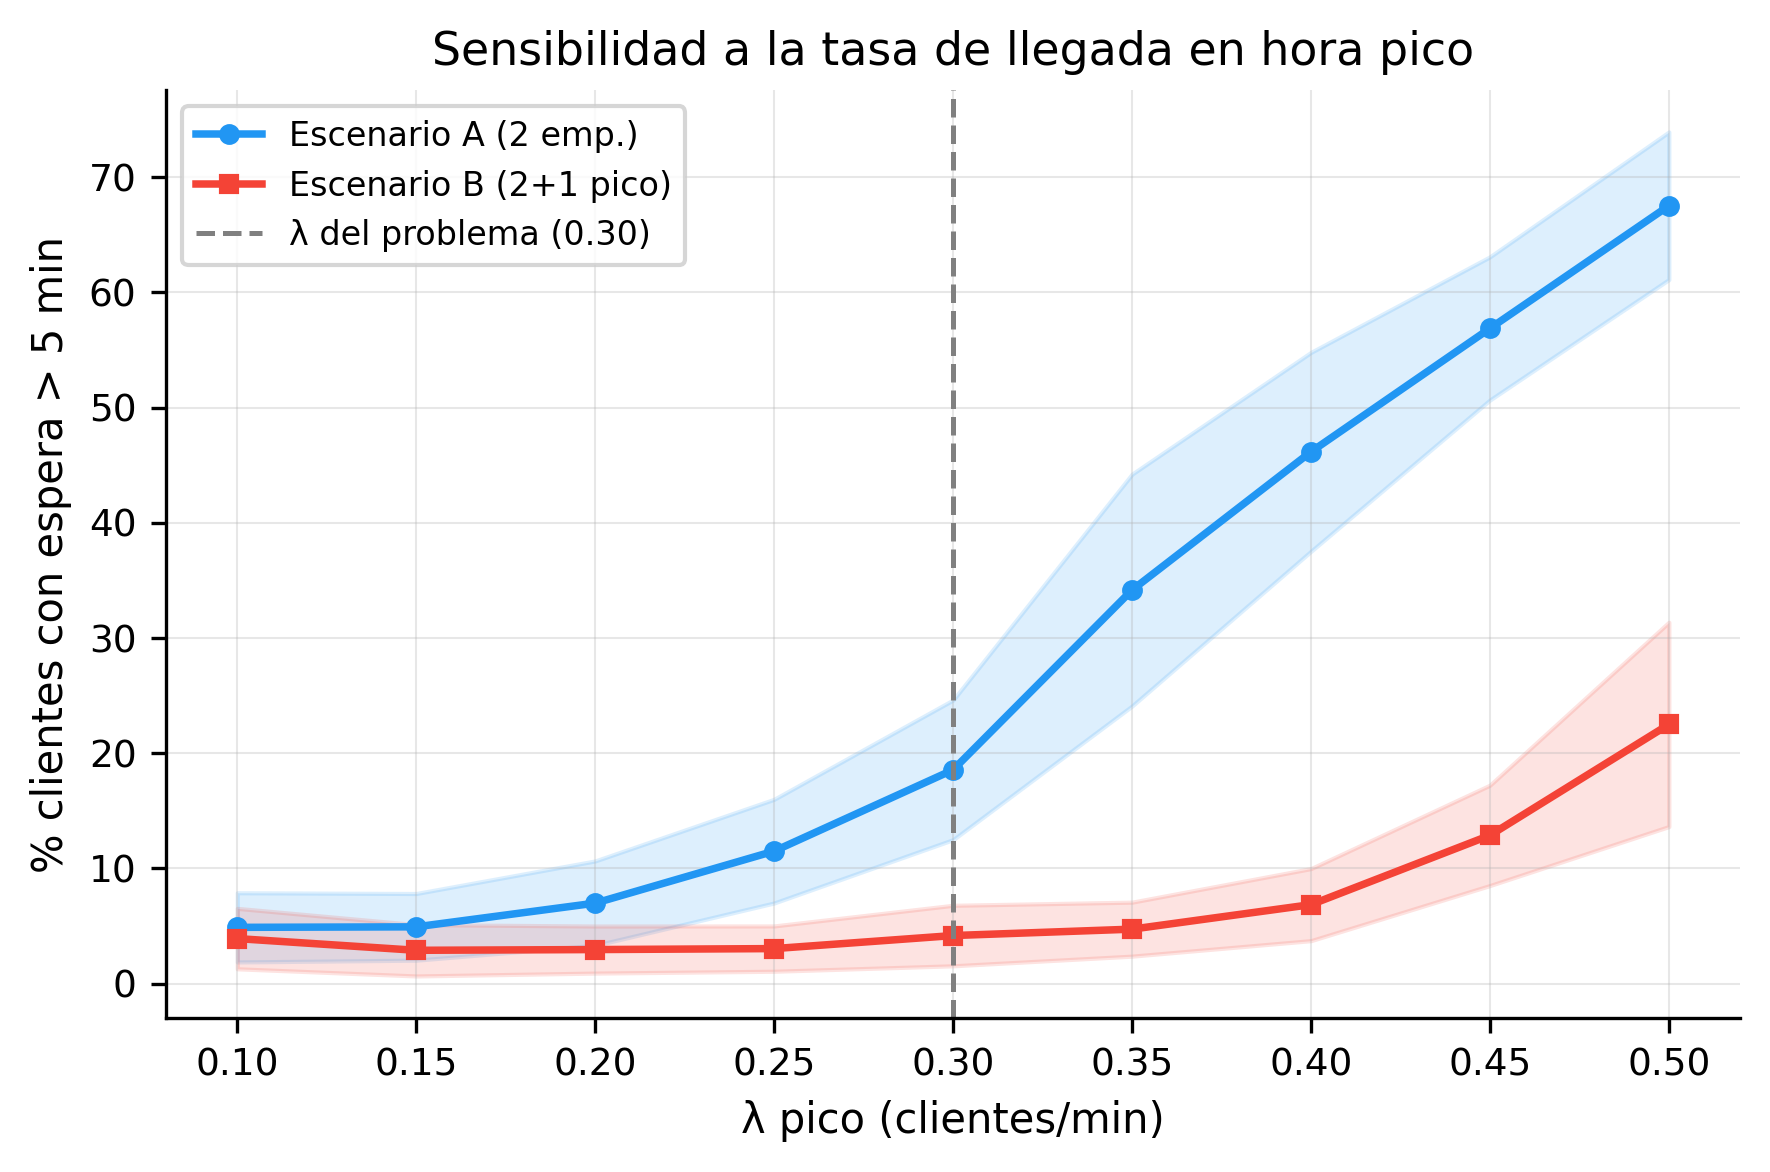
\includegraphics[width=0.85\linewidth]{figures/sensitivity.png}
  \caption{Sensibilidad del \% de clientes con espera $> 5$ min ante
           variaciones en $\lambda_{\text{peak}}$.
           La banda sombreada es el IC 95\,\%.
           La línea discontinua gris marca el valor nominal del problema
           ($\lambda = 0{,}30$).}
  \label{fig:sensibilidad}
\end{figure}

La \cref{fig:sensibilidad} revela varias conclusiones importantes:

\begin{itemize}
  \item Para $\lambda_{\text{peak}} \le 0{,}20$ clientes/min ambos escenarios
    presentan porcentajes de insatisfacción inferiores al 5\,\%;
    la inversión en personal extra no está justificada a esas tasas.
  \item En el valor nominal $\lambda = 0{,}30$, el Escenario B reduce el
    indicador de 16{,}7\,\% a 3{,}1\,\%.
  \item A partir de $\lambda_{\text{peak}} \approx 0{,}42$ el Escenario B
    también comienza a saturarse (supera el 10\,\%),
    indicando que para tasas más altas sería necesario incorporar un cuarto
    empleado durante las horas pico.
\end{itemize}

% ---------------------------------------------------------------------------
\subsection{Sensibilidad a la tasa de llegada fuera de hora pico}
% ---------------------------------------------------------------------------

Se analiza también el impacto de variaciones en la tasa de llegadas fuera de
las horas pico $\lambda_{\text{off-peak}}$.
Se ejecutan 10 réplicas por punto; los valores evaluados son
$\lambda_{\text{off-peak}} \in \{0{,}05;\;0{,}10;\;\ldots;\;0{,}35\}$,
manteniendo $\lambda_{\text{peak}} = 0{,}30$ y el resto de parámetros fijos.

\begin{figure}[H]
  \centering
  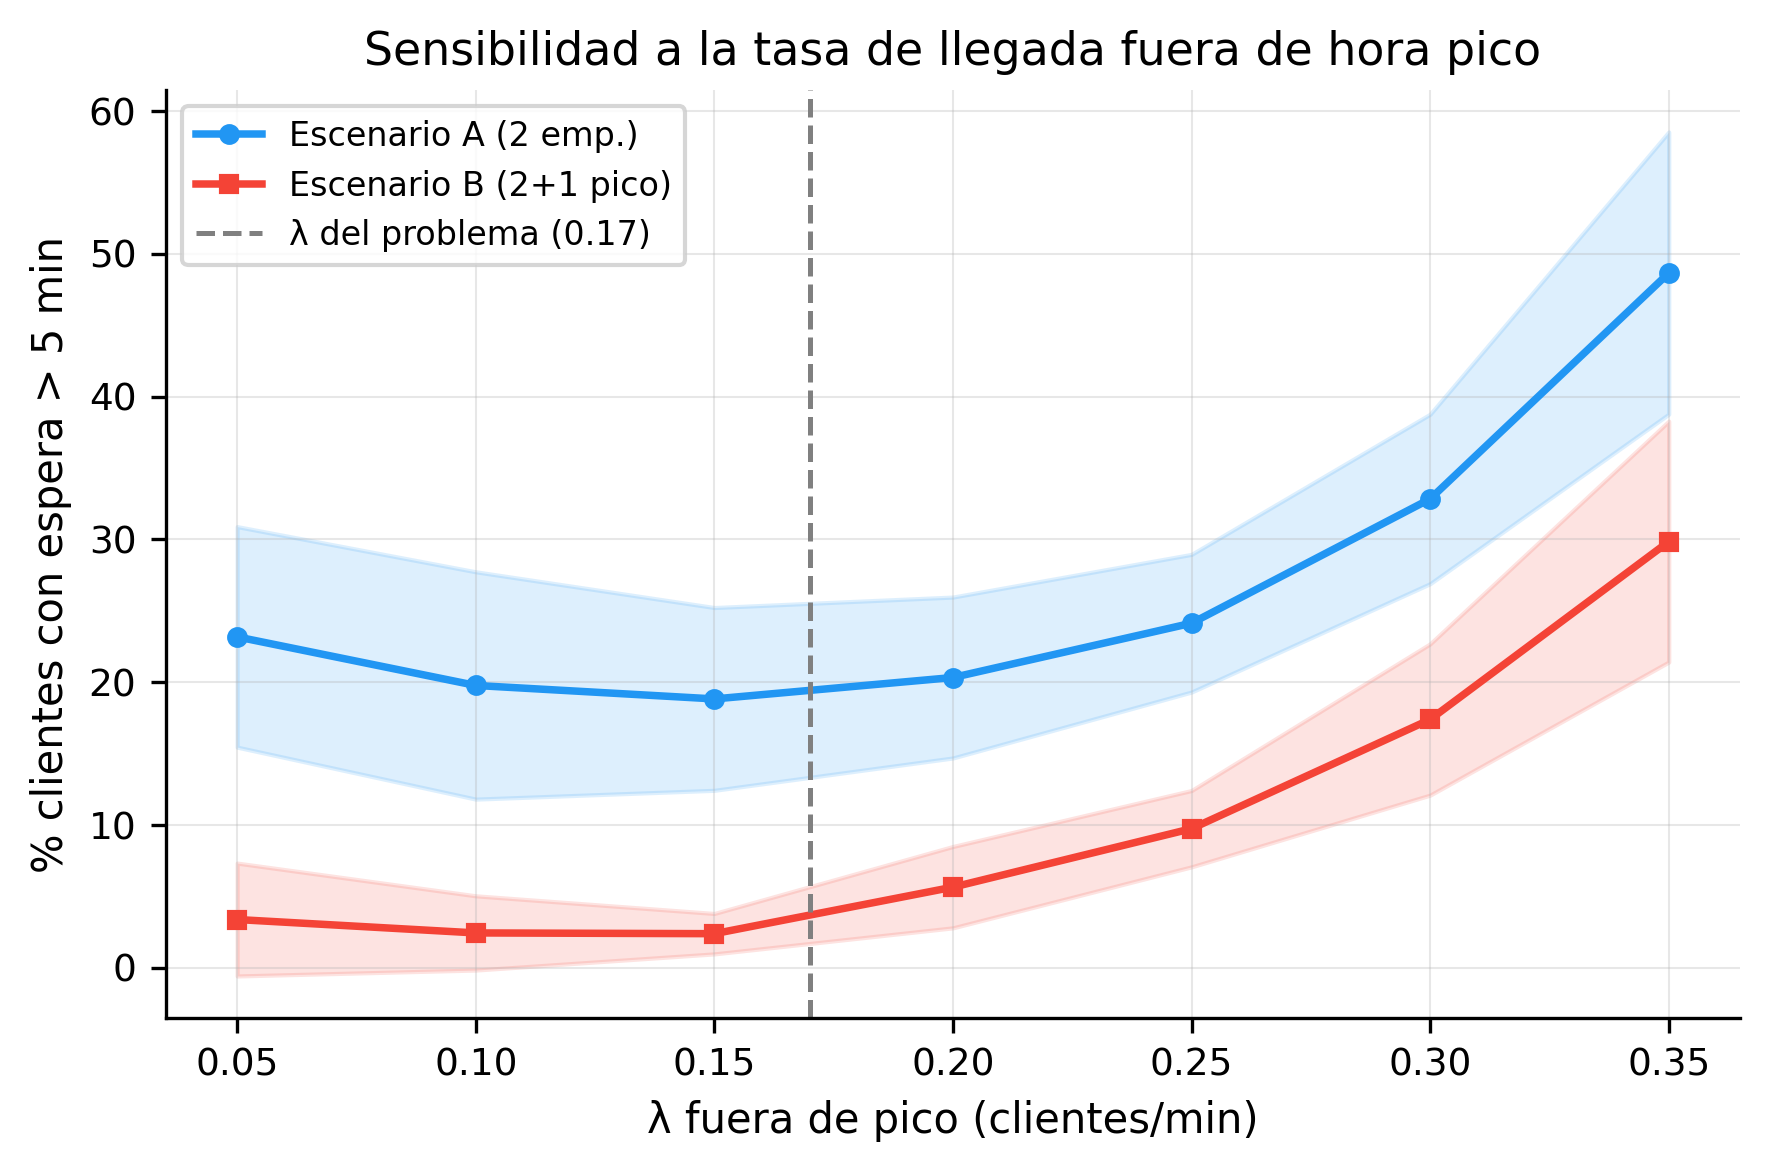
\includegraphics[width=0.85\linewidth]{figures/sensitivity_offpeak.png}
  \caption{Sensibilidad del \% de clientes con espera $> 5$ min ante
           variaciones en $\lambda_{\text{off-peak}}$.
           La banda sombreada es el IC 95\,\%.
           La línea discontinua gris marca el valor nominal
           ($\lambda_{\text{off-peak}} = 0{,}17$).}
  \label{fig:sensibilidad_fuera}
\end{figure}

La \cref{fig:sensibilidad_fuera} muestra que:
\begin{itemize}
  \item La tasa fuera de pico tiene un impacto moderado en comparación con
    $\lambda_{\text{peak}}$: incluso duplicando $\lambda_{\text{off-peak}}$
    desde 0{,}17 hasta 0{,}34, el incremento en el porcentaje de insatisfacción
    es notablemente menor que el producido por variaciones equivalentes en la
    tasa de pico.
  \item El Escenario B mantiene su ventaja frente a A en todo el rango analizado,
    lo que confirma que la recomendación de incorporar un tercer empleado en
    horas pico es robusta ante fluctuaciones en la demanda fuera de pico.
  \item Para $\lambda_{\text{off-peak}} \gtrsim 0{,}30$ clientes/min (valor
    comparable a la tasa de pico), el sistema comienza a saturarse incluso
    fuera de las horas pico, por lo que en ese régimen sería necesario revisar
    la dotación base de empleados.
\end{itemize}

\newpage
% =============================================================================
\section{Modelo Matemático}
% =============================================================================

% ---------------------------------------------------------------------------
\subsection{Clasificación del sistema de colas}
% ---------------------------------------------------------------------------

El sistema de La Cocina de Kojo puede clasificarse, usando la notación de
Kendall, como un sistema \textbf{M/G/$c$}:
\begin{itemize}
  \item \textbf{M} (Markoviano): las llegadas de clientes forman un proceso
    de Poisson, cuyos tiempos entre eventos son variables exponenciales
    independientes --- memoria nula entre llegadas sucesivas.
  \item \textbf{G} (General): los tiempos de servicio siguen distribuciones
    uniformes, no exponenciales.
  \item \textbf{$c$}: hay $c \in \{2, 3\}$ servidores paralelos con cola
    única FIFO.
\end{itemize}

Dado que la tasa de llegadas no es constante a lo largo del día, el modelo
global es en realidad un sistema M/G/$c$ \emph{no estacionario}.
El análisis teórico que sigue trata cada período (pico / fuera de pico) de
forma independiente asumiendo condiciones de régimen estacionario dentro de
cada tramo.

% ---------------------------------------------------------------------------
\subsection{Parámetros del servicio}
% ---------------------------------------------------------------------------

\paragraph{Tiempo de servicio esperado.}
Con probabilidad $p = 0{,}5$ el cliente pide sándwich
($S_{\text{sand}} \sim \mathcal{U}[3,5]$) y con probabilidad $1-p = 0{,}5$
pide sushi ($S_{\text{sush}} \sim \mathcal{U}[5,8]$).
La esperanza del tiempo de servicio es:
\begin{equation}
  \EE[S] = p\,\EE[S_{\text{sand}}] + (1-p)\,\EE[S_{\text{sush}}]
         = 0{,}5 \cdot \frac{3+5}{2} + 0{,}5 \cdot \frac{5+8}{2}
         = 0{,}5 \times 4 + 0{,}5 \times 6{,}5
         = \mathbf{5{,}25} \text{ min.}
  \label{eq:ES}
\end{equation}

La tasa de servicio de un empleado es:
\[
  \mu = \frac{1}{\EE[S]} = \frac{1}{5{,}25} \approx 0{,}1905 \text{ clientes/min.}
\]

\paragraph{Segundo momento y varianza del servicio.}
Para $X \sim \mathcal{U}[a,b]$ se tiene
$\EE[X^2] = (a^2 + ab + b^2)/3$.
Por tanto:
\[
  \EE[S_{\text{sand}}^2] = \frac{9 + 15 + 25}{3} = \frac{49}{3} \approx 16{,}33, \qquad
  \EE[S_{\text{sush}}^2] = \frac{25 + 40 + 64}{3} = 43.
\]
\[
  \EE[S^2] = 0{,}5 \times \frac{49}{3} + 0{,}5 \times 43
           = 8{,}167 + 21{,}5 = \mathbf{29{,}67} \text{ min}^2.
\]
\[
  \VV[S] = \EE[S^2] - (\EE[S])^2 = 29{,}67 - 5{,}25^2 = 29{,}67 - 27{,}5625
         \approx \mathbf{2{,}11} \text{ min}^2, \quad
  \sigma_S \approx 1{,}45 \text{ min.}
\]

% ---------------------------------------------------------------------------
\subsection{Utilización teórica y estabilidad}
% ---------------------------------------------------------------------------

La \textbf{utilización} de cada servidor en el período analizado es:
\begin{equation}
  \rho = \frac{\lambda}{c \cdot \mu},
  \label{eq:rho}
\end{equation}
con la condición de estabilidad $\rho < 1$.
La \cref{tab:utilizacion_teorica} muestra los valores para cada combinación
de período y escenario.

\begin{table}[H]
  \centering
  \caption{Utilización teórica $\rho$ por período y escenario.}
  \label{tab:utilizacion_teorica}
  \begin{tabular}{llcccc}
    \toprule
    \textbf{Período} & \textbf{Escenario} & $\lambda$ & $c$ & $\mu$ & $\rho = \lambda/(c\mu)$ \\
    \midrule
    Fuera de pico & A & 0{,}17 & 2 & 0{,}1905 & 0{,}446 \\
    Fuera de pico & B & 0{,}17 & 2 & 0{,}1905 & 0{,}446 \\
    Pico          & A & 0{,}30 & 2 & 0{,}1905 & 0{,}787 \\
    Pico          & B & 0{,}30 & 3 & 0{,}1905 & 0{,}525 \\
    \bottomrule
  \end{tabular}
\end{table}

En todos los casos $\rho < 1$: el sistema es estable en cada período.
La carga más exigente corresponde al período pico del Escenario A ($\rho =
0{,}787$), lo que explica la acumulación de cola observada en la simulación.

% ---------------------------------------------------------------------------
\subsection{Aproximación M/M/c como cota teórica}
% ---------------------------------------------------------------------------

Para obtener predicciones analíticas se aproxima el sistema M/G/$c$ por un
sistema M/M/$c$ con la misma tasa media de servicio.
Aunque los tiempos de servicio no son exponenciales, este modelo proporciona
una cota de referencia útil.

\paragraph{Fórmula de Erlang~C.}
La probabilidad de que un cliente deba esperar en cola es~\citep{banks2010discrete}:
\begin{equation}
  C(c,\,a) = \frac{\displaystyle\frac{a^c}{c!}\cdot\frac{c}{c - a}}
                  {\displaystyle\sum_{n=0}^{c-1}\frac{a^n}{n!}
                   + \frac{a^c}{c!}\cdot\frac{c}{c - a}},
  \label{eq:erlangC}
\end{equation}
donde $a = \lambda/\mu$ es la intensidad de tráfico.

\paragraph{Tiempo de espera en cola (M/M/$c$).}
\begin{equation}
  W_q^{\text{MM}c} = \frac{C(c,\,a)}{c\,\mu\,(1-\rho)}.
  \label{eq:Wq_mmc}
\end{equation}

\paragraph{Longitud media de cola.}
Por la Ley de Little~\citep{little1961proof}:
\begin{equation}
  L_q = \lambda\,W_q.
  \label{eq:little}
\end{equation}

Los resultados se muestran en la \cref{tab:teoria_vs_sim}.
Los valores teóricos se calculan como media ponderada por tiempo de los dos períodos
del día: $W_q^{\text{día}} = \frac{240}{660}\,W_q^{\text{pico}} + \frac{420}{660}\,W_q^{\text{fuera}}$,
con $\lambda_{\text{eff}} = \frac{240 \times 0{,}30 + 420 \times 0{,}17}{660} = 0{,}217$ clientes/min.

\begin{table}[H]
  \centering
  \caption{Comparación teoría M/M/$c$ vs.\ simulación ---
           media ponderada del día completo.}
  \label{tab:teoria_vs_sim}
  \begin{tabular}{llccc}
    \toprule
    \textbf{Escenario} & \textbf{Indicador}
      & \textbf{M/M/$c$ teórico}
      & \textbf{Simulación (media)}
      & \textbf{Sim $-$ Teo (\%)} \\
    \midrule
    A ($c_{\text{pico}}=2$) & $W_q$ (min)      & 3{,}95 & 2{,}19 & $-$44{,}6 \\
    A ($c_{\text{pico}}=2$) & $L_q$ (clientes) & 0{,}86 & 0{,}48 & $-$44{,}2 \\
    B ($c_{\text{pico}}=3$) & $W_q$ (min)      & 1{,}18 & 0{,}66 & $-$44{,}1 \\
    B ($c_{\text{pico}}=3$) & $L_q$ (clientes) & 0{,}26 & 0{,}15 & $-$42{,}3 \\
    \bottomrule
  \end{tabular}
\end{table}

% ---------------------------------------------------------------------------
\subsection{Supuestos, restricciones y fuentes de discrepancia}
% ---------------------------------------------------------------------------

Las diferencias entre el modelo M/M/$c$ y la simulación se explican por
varios factores:

\begin{enumerate}
  \item \textbf{Distribución del servicio (factor dominante).}
    Los tiempos de servicio son uniformes, no exponenciales.
    La distribución exponencial tiene coeficiente de variación $C_v = 1$,
    mientras que $\mathcal{U}[3,5]$ tiene $C_v = 0{,}14$,
    $\mathcal{U}[5,8]$ tiene $C_v = 0{,}13$, y la mezcla combinada tiene
    $C_v = \sigma_S / \EE[S] = 1{,}45 / 5{,}25 \approx 0{,}28$.
    Tiempos de servicio mucho menos variables que los exponenciales generan
    colas notablemente menores, como predice la fórmula de
    Pollaczek--Khinchine~\citep{ross2013simulation}.
    Este factor explica que la simulación dé resultados aprox.\ \SI{44}{\percent}
    menores que M/M/$c$ de manera consistente en ambos escenarios.

  \item \textbf{No estacionariedad.}
    La tasa $\lambda(t)$ cambia a lo largo del día.
    El modelo estacionario sobreestima el efecto del pico porque asume que la
    tasa alta ha estado vigente indefinidamente, acumulando más cola de la real.

  \item \textbf{Condición transitoria.}
    Al inicio de cada período pico el sistema parte de una cola residual, no del
    estado de régimen estacionario que asume el modelo analítico.

  \item \textbf{Jornada finita.}
    La Ley de Little y la fórmula de Erlang C son resultados de largo plazo
    (régimen estacionario); aquí el horizonte es de 660 min.
\end{enumerate}

\paragraph{Verificación con la Ley de Little.}
Se puede verificar internamente la consistencia de la simulación usando
$L_q = \lambda_{\text{eff}}\,W_q$, donde $\lambda_{\text{eff}}$ es la tasa
efectiva de clientes atendidos.
Para el Escenario A: $0{,}482 \approx (144{,}2 / 660) \times 2{,}185 = 0{,}218 \times 2{,}185 = 0{,}477$ $\checkmark$

\newpage
% =============================================================================
\section{Conclusiones}
% =============================================================================

\subsection{Recomendación principal}

La simulación de 30 réplicas por escenario, emparejadas mediante números
aleatorios comunes, proporciona evidencia estadística abrumadora ($p = 1{,}12 \times 10^{-11}$,
$t = 10{,}8$, IC de la diferencia $[11{,}03;\;16{,}18]$ pp) de que incorporar
un tercer empleado durante las horas pico reduce el porcentaje de clientes
con espera superior a 5 minutos de \textbf{16{,}7\,\%} (Escenario A) a
\textbf{3{,}1\,\%} (Escenario B), una mejora del 81{,}4\,\%.

Se \textbf{recomienda adoptar el Escenario B} para la tasa de llegadas actual
($\lambda_{\text{pico}} = 0{,}30$ clientes/min).

\subsection{Hallazgos secundarios}

\begin{itemize}
  \item El tiempo de espera medio se reduce de 2{,}19 min a 0{,}66 min.
  \item La longitud media de la cola decrece de 0{,}48 a 0{,}15 clientes.
  \item La utilización del personal baja del 57{,}2\,\% al 50{,}2\,\%,
    manteniéndose en niveles saludables que permiten absorber picos
    transitorios sin colapsar el sistema.
  \item El análisis de sensibilidad revela que la ventaja del Escenario B
    se mantiene para $\lambda_{\text{pico}} \lesssim 0{,}42$; por encima de
    ese umbral sería necesario incorporar un cuarto empleado.
\end{itemize}

\subsection{Limitaciones del modelo}

\begin{enumerate}
  \item \textbf{Disciplina de cola:} se asume FIFO estricto; no se modela
    abandono (reneging) ni impaciencia de los clientes.
  \item \textbf{Homogeneidad de empleados:} todos los servidores tienen la
    misma distribución de servicio; no se considera variabilidad inter-empleado.
  \item \textbf{Jornada determinista:} el horario de apertura y cierre, y las
    fronteras de hora pico, son fijas.
    En la práctica pueden fluctuar.
  \item \textbf{Sin descansos ni ausencias:} el modelo asume disponibilidad
    continua de los empleados.
  \item \textbf{Modelo no estacionario aproximado:} la generación de llegadas
    usa tasas constantes por tramos, no un proceso de Poisson no homogéneo
    exacto.
\end{enumerate}

\subsection{Posibles extensiones}

\begin{itemize}
  \item Incorporar abandono de cola: modelar que los clientes se van si
    la espera estimada supera un umbral.
  \item Optimizar el número óptimo de empleados extra como función de
    $\lambda_{\text{pico}}$, generalizando el análisis de sensibilidad.
  \item Ajustar las distribuciones de servicio a datos reales del local
    (análisis de bondad de ajuste).
  \item Extender el análisis de parada usando métodos secuenciales
    (semi-anchura fija) para garantizar el criterio del 5\,\% de precisión
    relativa~\citep{law2015simulation}.
\end{itemize}


% ── Bibliografía ──────────────────────────────────────────────────────────────
\newpage
\bibliographystyle{plainnat}
\bibliography{references}

\end{document}
